\begin{frame}
    \begin{columns}[c]
        \column{.5\textwidth}
        
        General intro here
        
        \column{.5\textwidth}

        \begin{figure}
            \begin{center}
            \includegraphics[width=\textwidth]{../images/darwin-tol-copyright-boris-kulikov-2007.jpg}
            \caption{\tiny \copyright~2007 Boris Kulikov \href{http://boris-kulikov.blogspot.com/}{boris-kulikov.blogspot.com}}
            \end{center}
        \end{figure}
    \end{columns}
\end{frame}

{
\setbeamercolor{background canvas}{bg=black}
\setbeamercolor{whitetext}{fg=white}
\begin{frame}
    \frametitle{Processes of diversification}
    \begin{columns}[c]
        \column{.5\textwidth}
        {\usebeamercolor[fg]{whitetext}
        \begin{itemize}
            \item<2-> Large-scale geological and climatic processes are
                important in biodiversification and community assembly
            \item<3-> Accounting for such processes will better our
                understanding of biodiversity
            \item<4-> We need methods for inferring evolutionary patterns
                predicted by historical events from contemporary populations
        \end{itemize}
        }
        \column{.5\textwidth}
        \begin{figure}
            \begin{center}
            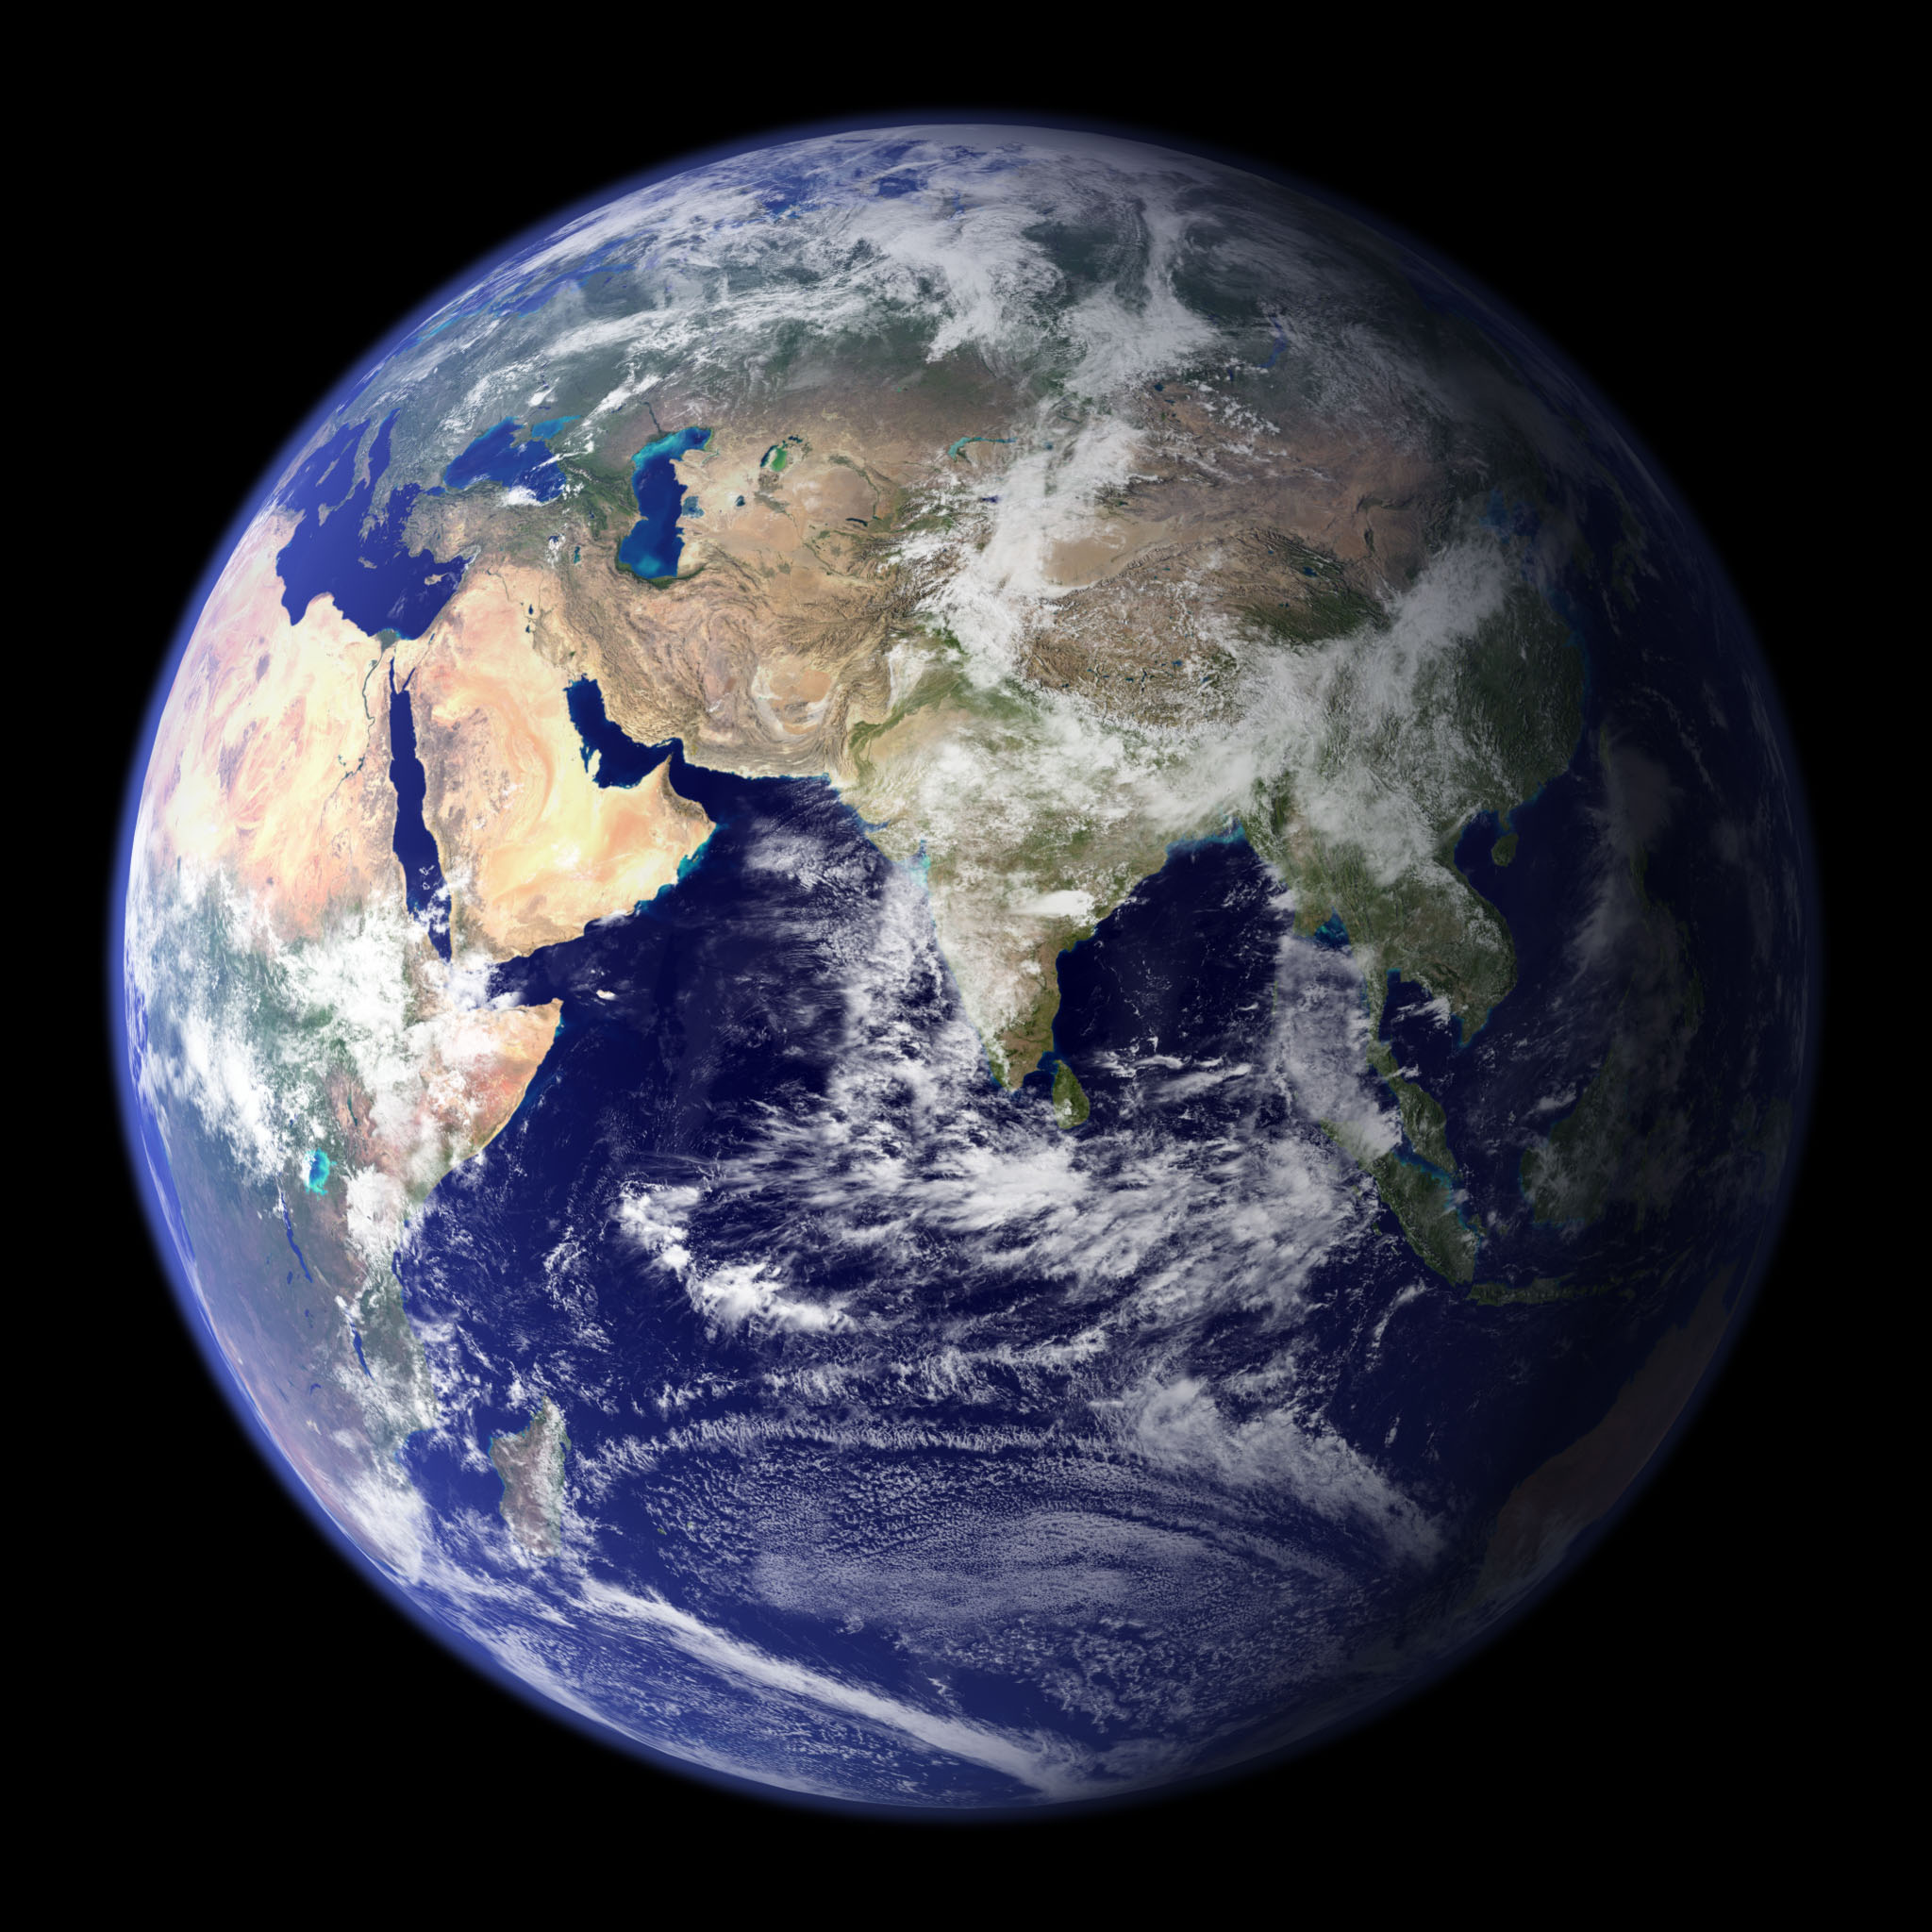
\includegraphics[width=\textwidth]{../images/earth-image.jpg}
            \end{center}
        \end{figure}
    \end{columns}
\end{frame}
}

